\section{Software Implementation with SciKit-Surgery}
%these commands might work on some systems if you have -shell-escape set but I couldn't get it working on overleaf
%\immediate\write18{wget https://glenoidplanefitting.readthedocs.io/en/latest/_images/graphviz-f4a0d46f29de525cf2512540ebd2f3e3f3356594.png}
%\input|"wget https://glenoidplanefitting.readthedocs.io/en/latest/_images/graphviz-f4a0d46f29de525cf2512540ebd2f3e3f3356594.png"
\sksglenoid is built on top of the \sksurgery \cite{PMID:32436132} libraries which enabled
rapid development and future deployment into a clinically useable application. 
Development was kick started using the \sksurgery Python Template \cite{doel_tom_2022_5879146} enabling the bulk of the development and testing to be performed during a 10 week summer internship with minimal prior experience of Python or software development. \sksurgery also includes template libraries for C++ projects \cite{dowrick2021cmakecatchtemplate}.

\sksurgery is made up of multiple Python libraries and currently supports clinical 
guidance systems \cite{schneider2020comparison}, research platforms for registration \cite{thompson2021fiducial} and ultrasound simulation \cite{thompson2020snappysonic}. 
Figure \ref{fig:deps} shows the immediate dependencies of \sksglenoidns. The most significant dependencies are NumPy\cite{2020NumPy-Array} which is used for the version calculation, and {VTK}\cite{Schroeder:1998:VTO:272980} which is used for visualising the results. SciKit-SurgeryCore provides configuration helpers for the user interface. SciKit-SurgeryVTK provides some helpful loaders and shape primitives, but it may be useful to remove this dependency as it would significantly simplify the dependency graph.

\begin{figure}
	\begin{center}
		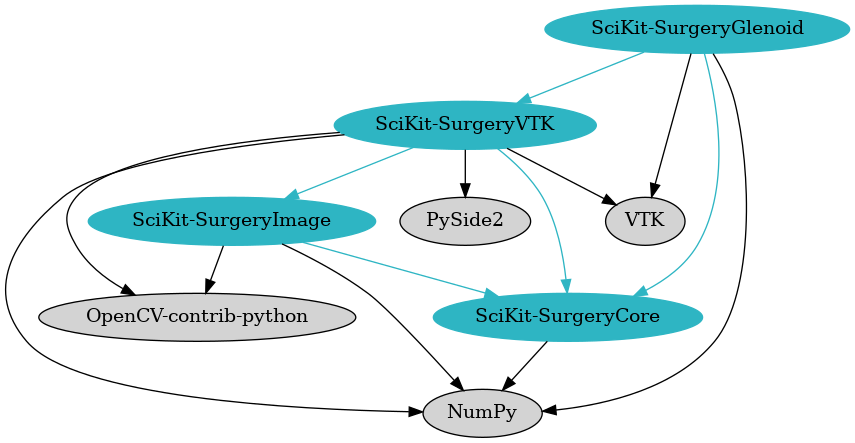
\includegraphics[width=0.6\linewidth]{figures/dep_graph.png}
			\caption{\label{fig:deps}The dependency graph for SciKit-SurgeryGlenoid. SciKit-Surgery dependencies are shown in blue, whilst 3rd party dependencies are shown in grey.}
	\end{center}
\end{figure}
